%% This is file `elsarticle-template-1-num.tex',
%%
%% Copyright 2009 Elsevier Ltd
%%
%% This file is part of the 'Elsarticle Bundle'.
%% ---------------------------------------------
%%
%% It may be distributed under the conditions of the LaTeX Project Public
%% License, either version 1.2 of this license or (at your option) any
%% later version.  The latest version of this license is in
%%    http://www.latex-project.org/lppl.txt
%% and version 1.2 or later is part of all distributions of LaTeX
%% version 1999/12/01 or later.
%%
%% The list of all files belonging to the 'Elsarticle Bundle' is
%% given in the file `manifest.txt'.
%%
%% Template article for Elsevier's document class `elsarticle'
%% with numbered style bibliographic references
%%
%% $Id: elsarticle-template-1-num.tex 149 2009-10-08 05:01:15Z rishi $
%% $URL: http://lenova.river-valley.com/svn/elsbst/trunk/elsarticle-template-1-num.tex $
%%
\documentclass[preprint,12pt]{elsarticle}

%% Use the option review to obtain double line spacing
%% \documentclass[preprint,review,12pt]{elsarticle}

%% Use the options 1p,twocolumn; 3p; 3p,twocolumn; 5p; or 5p,twocolumn
%% for a journal layout:
%% \documentclass[final,1p,times]{elsarticle}
%% \documentclass[final,1p,times,twocolumn]{elsarticle}
%% \documentclass[final,3p,times]{elsarticle}
%% \documentclass[final,3p,times,twocolumn]{elsarticle}
%% \documentclass[final,5p,times]{elsarticle}
%% \documentclass[final,5p,times,twocolumn]{elsarticle}

%% if you use PostScript figures in your article
%% use the graphics package for simple commands
%% \usepackage{graphics}
%% or use the graphicx package for more complicated commands
%% \usepackage{graphicx}
%% or use the epsfig package if you prefer to use the old commands
%% \usepackage{epsfig}

%% The amssymb package provides various useful mathematical symbols
\usepackage{amssymb}
%% The amsthm package provides extended theorem environments
%% \usepackage{amsthm}

%% The lineno packages adds line numbers. Start line numbering with
%% \begin{linenumbers}, end it with \end{linenumbers}. Or switch it on
%% for the whole article with \linenumbers after \end{frontmatter}.
\usepackage{lineno}

%% natbib.sty is loaded by default. However, natbib options can be
%% provided with \biboptions{...} command. Following options are
%% valid:

%%   round  -  round parentheses are used (default)
%%   square -  square brackets are used   [option]
%%   curly  -  curly braces are used      {option}
%%   angle  -  angle brackets are used    <option>
%%   semicolon  -  multiple citations separated by semi-colon
%%   colon  - same as semicolon, an earlier confusion
%%   comma  -  separated by comma
%%   numbers-  selects numerical citations
%%   super  -  numerical citations as superscripts
%%   sort   -  sorts multiple citations according to order in ref. list
%%   sort&compress   -  like sort, but also compresses numerical citations
%%   compress - compresses without sorting
%%
%% \biboptions{comma,round}

% \biboptions{}
\usepackage{float}
\usepackage{booktabs}
\usepackage{multirow}

\journal{Environmental and Ecological Modelling}

\begin{document}


\begin{frontmatter}

%% Title, authors and addresses

%% use the tnoteref command within \title for footnotes;
%% use the tnotetext command for the associated footnote;
%% use the fnref command within \author or \address for footnotes;
%% use the fntext command for the associated footnote;
%% use the corref command within \author for corresponding author footnotes;
%% use the cortext command for the associated footnote;
%% use the ead command for the email address,
%% and the form \ead[url] for the home page:
%%
%% \title{Title\tnoteref{label1}}
%% \tnotetext[label1]{}
%% \author{Name\corref{cor1}\fnref{label2}}
%% \ead{email address}
%% \ead[url]{home page}
%% \fntext[label2]{}
%% \cortext[cor1]{}
%% \address{Address\fnref{label3}}
%% \fntext[label3]{}

\title{Spatial modelling of rice yield losses in Tanzania due to bacterial blight and leaf blast in a changing climate} 

%% use optional labels to link authors explicitly to addresses:
%% \author[label1,label2]{<author name>}
%% \address[label1]{<address>}
%% \address[label2]{<address>}

\author[AfricaRice]{C. Duku}
\ead{confidence.duku@wur.nl}
\author[IRRI]{A.H. Sparks}
\ead{a.sparks@irri.org}
\author[AfricaRice]{S.J. Zwart\corref{cor1}}
\ead{s.zwart@cgiar.org}
\author[IRRI]{J.K. Aunario}
\ead{j.aunario@irri.org}

\cortext[cor1]{Corresponding author}

\fntext[fn1]{Current address: Environmental Systems Analysis Group, Wageningen University, P.O. Box 47, 6700 AA Wageningen, The Netherlands} 
\address[AfricaRice]{Africa Rice Center (AfricaRice), 01 BP 2031, Cotonou, BENIN}
\address[IRRI]{International Rice Research Institute (IRRI), DAPO Box 7777, Metro Manila, 1301, PHILIPPINES}

\begin{abstract}

\end{abstract}

\begin{keyword}
bacterial blight \sep leaf blast \sep EPIRICE \sep RICEPEST \sep crop modelling\sep yield loss modelling
\end{keyword}

\end{frontmatter}



%%
%% Start line numbering here if you want
%%
\linenumbers

%% main text
\section{Software and data availability}
All code used for analysis and data used in this dataset are also available from Figshare ...url... and GitHub ...url... A Stella version of the original RICEPEST model by the original authors, Willocquet and Savary, is available for download from https://www.apsnet.org/edcenter/advanced/topics/BotanicalEpidemiology/Pages/default.aspx.


\section{Introduction}
Rice is the most rapidly growing staple food in Africa and although rice production is steadily increasing, the consumption is still out-pacing the production. For example by 2009 37 per cent of the rice consumed in Africa was imported. To reduce its reliance on imports and dependency on global markets Africa's rice production needs to increase further \cite{Seck2013}. Current average yield levels in Africa range from about 1 t ha\textsuperscript{-1} in upland ecologies to 1.5 to 2 t ha\textsuperscript{-1} in rainfed lowland ecologies with the irrigated lowland ecologies having the highest yields of 3.0 to 4.0 t ha\textsuperscript{-1} \cite{Diagne2013}. Rice yields in African farmers fields are low due to a combination of abiotic and biotic stresses that constrain them. Farmers can significantly reduce the yield gaps with improved field, water and crop management, and weed control \cite{Saito2013}.

Apart from weeds, pests and diseases also are major biotic stresses that can cause significant reductions in rice yields. Two important diseases in rice are leaf blast (LB), causal agent \textit{Magnaporthe oryzae}, and bacterial blight (BB) \cite{Verdier2012}, causal agent \textit{Xanthamonas oryzae} pv. \textit{oryzae}. Because infectious plant disease occurs as an interaction of a favorable environment, a susceptible host and a competent pathogen \cite{Madden2007}, weather conditions impact both the occurrence and gravity of plant disease. Climate change is likely to affect plant disease \cite{Anderson2004, Coakley1999, Garrett2006} and several others have expressed interest in changes to plant disease as a result of climate change \cite{Chakraborty2011, Juroszek2011, Luck2011, Pautasso2010, Savary2011, Sutherst2011}. Moreover, intensification of rice production, which was witnessed in Sub-Saharan Africa since the food crisis of 2008 \cite{Saito2013}, may lead to an increased yield loss due to the blast, thus reducing the benefits that were created \cite{Sere2013}. Increases in disease incidence and severity may deter farmers from investing in intensification measures because of risks related to yield losses or even total crop failure. To the authors knowledge, the impact of climate change on leaf blast and bacterial blight diseases of rice in Africa has not yet been investigated.

Efforts to link plant disease models with a geographic information system (GIS) to assess the impact of plant diseases spatially include  \citet{Hijmans2000}, which mapped the global number of pesticide applications necessary to control potato late blight using contemporary weather data. While \citet{Sparks2014} used a meta-model to generate map estimates of changes in global potato late blight due to climate change. \citet{Savary2012} developed a GIS-linked model, EPIRICE, capable of simulating several important diseases of rice, including leaf blast and bacterial blight amongst others.

The objective of the study was to quantify the impact of climate change as forecast by the Intergovernmental Panel on Climate Change (IPCC) on rice yield loss as result of BB and LB. To carry out this study, we linked two previously unlinked, existing models, EPIRICE and RICEPEST \cite{Willocquet2000, Willocquet2002}, and we applied them using spatially and temporally downscaled climate change data to generate predictions on changes in plant disease impact due to climate change in Tanzania.

Rice accounts for five percent of the total value of agricultural production in Tanzania and is the seventh most important agricultural crop with steadily increasing production over the last decade. However, rice yields in Tanzania remain significantly lower than in neighboring countries \cite{Barreiro-Hurle2012}.

The linkage of EPIRICE with RICEPEST gives two advantages. First, RICEPEST has been used to estimate yield losses due to diseases and other pest injuries in rice in varying production situations with current weather and climate conditions. However, as plant diseases are affected by weather, the linkage with EPIRICE allows us to model the effects of climate change on both the rice crop and on the diseases while using the same weather data inputs. Second, the spatial nature of EPIRICE outputs enabled us to use RICEPEST in a GIS. Until now RICEPEST yield loss estimates have not been linked to a GIS. Linking RICEPEST with a GIS allowed us to map yield losses for the whole country of Tanzania, rather than just point based predictions of yield losses.

This paper will continue with a justification for the study area, followed by descriptions of the EPIRICE and RICEPEST models. We will then elaborate the framework for assessing rice yield losses under climate change that links both models. The procedure for generating daily weather inputs from the downscaled climate scenarios is outlined followed by the choice of production situations. Next the results are presented, followed by a discussion and finally conclusions.

\section{Materials and Methods}

%Rice (importance, areas, growing seasons)
%Current climate 
%Climate change impact (growing seasons?)

\subsection{The study region}
Tanzania was chosen as the study region because of its location in sub-Saharan Africa, the probable effects of climate change in the region and rice is planted widely across the country \cite{Rowhani2011} (Table 1). The bulk of the rice crop is grown from December until June of the following year during the rainy season. 

According to the International Panel on Climate Change (IPCC), East Africa and especially the Great Lakes Region are among the more vulnerable regions in Africa to climate change, where the trend is towards increasing temperatures and declining rainfall according to General Circulation Model outputs \cite{Boko2007}. Temperatures are predicted to increase 2 $^{\circ}$C by 2050, which in turn are predicted to negatively affect rice yields \cite{Rowhani2011}.

\subsection{Model descriptions}
\subsubsection{The EPIRICE model}
EPIRICE \cite{Savary2012} is a SEIR (susceptible-exposed-infectious-removed) model \cite{Kermack1927, Madden2006} implemented in R \cite{R2014} that simulates potential spatial epidemics of rice diseases including BB and LB. The model considers a 1m\textsuperscript{2} area of rice, which is the same area that RICEPEST considers. Model inputs are date of crop establishment and daily time-step weather data; precipitation, maximum and minimum temperature, and relative humidity. The model as originally implemented produces a single aggregated output, a map, at the end of a growing season of a measure called Area Under Disease Progress Curve (AUDPC) \cite{Shaner1977}. However, for this study, daily disease severity expressed as a percentage was generated for use in the RICEPEST model, which we discuss further in a later portion of this paper. As the only modification made to the model was the expression of daily disease severity, we  would refer the reader to \citet{Savary2012} for further information on the model structure and function.

\subsubsection{The RICEPEST model}
The RICEPEST model \cite{Willocquet2000, Willocquet2002} simulates rice yield losses due to several yield-reducing factors under a range of specific production situations with simulated diseases including BB and LB. The model runs on a daily time-step with simulation starting 14 days after crop establishment (DACE) for both transplanted and direct seeded rice. The model incorporates two sub-models, the first sub-model simulates the dynamics of the rice crop biomass and the second sub-model simulates the dynamics of the tiller population. The biomass sub-model accounts for the daily accumulation and partitioning of assimilates towards roots, leaves, stems, and panicles. For this study, because the damage mechanisms of the diseases of interest (BB and LB) are simulated only in the biomass sub-model, the tiller sub-model was not considered.

Bacterial blight and LB cause lesions on the leaf blades. These lesions decrease the green leaf area index (LAI), reducing the photosynthetic capacity of the plant. RICEPEST reduces the rate of growth (RG) (Formula \ref{RG}) by reducing the LAI (Formula \ref{LAI}) by applying a damage function (Formula \ref{BBDM}) or (\ref{LBDM}) where SLA is the specific leaf area; LEAFW is the leaf dry weight; RUE is radiation use efficiency; RAD is daily solar radiation; k is coefficient of light extinction and is defined as the proportion of light intercepted by the crop \cite{Willocquet2000}, set to 0.6 \cite{Willocquet2002}.
\begin{equation}\label{RG}
RG_t = RUE_t \times RAD_t \times (1- exp(- k \times LAI_t))
\end{equation}

\begin{equation}\label{LAI}
LAI_t = SLA_t \times LEAFWt
\end{equation}
The damage functions that calculate the reduction factors, BBDM (Formula \ref{BBDM}) and LBDM (Formula \ref{LBDM}) are the percent of leaf area covered by BB and LB respectively \cite{Willocquet2002}. 
\begin{equation}\label{BBDM}
(1-(BBDM_t /100)
\end{equation}

\begin{equation}\label{LBDM}
(1-(LBDM_t /100))
\end{equation}
Thus, the complete LAI formula with the damage function for BB reducing the photosynthetic area of the leaf becomes
 \begin{equation}\label{LAIBBDM}
LAI_t = SLA_t \times LEAFWt \times (1-(BBDM_t / 100)).
\end{equation}

\subsubsection{Model coupling}
To facilitate coupling of EPIRICE to RICEPEST, a temporal disaggregation function was incorporated into the EPIRICE model. With this function, the modified EPIRICE model produced daily, spatially representative and non-cumulative percentage disease severity data as outputs instead of the single cumulated output, AUDPC. The time-series of daily percentage disease severity data for BB and LB produced by the modified EPIRICE model were then used as inputs for RICEPEST. Both models were linked to a geographic information system (GIS). EPIRICE is implemented in the R language using the following packages: cropsim \cite{Hijmans2009}, oldweather \cite{Hijmans2009}, raster \cite{Hijmans2014}, rgdal \cite{Bivand2014}, and RODBC \cite{Ripley2013}, while this version of RICEPEST is implemented in Python language \cite{python}, using the ArcPy package, as a script in the ArcGIS platform \cite{ESRI2011}. Due to the different implementation environments, a loose coupling approach was therefore adopted. A loose coupling approach provided flexibility in data handling and data interoperability. 

\subsection{Growing seasons and areas}
The major planting window in Tanzania for most rain-fed ecologies in Tanzania according to the IRRI rice cropping calendar (citation) was October to December, with the largest area of Tanzania being planted in late November (Figshare citation). Because the original climate data were monthly, not daily and needed to be temporally downscaled, a planting window of late November to early December was selected and ArcGIS was used to create a spatial dataset of areas with this planting window. Annual harvested rain-fed rice growing areas for Tanzania with values representing the proportion of harvested areas (in hectares) within each pixel (10,000ha) was also obtained from MIRCA2000 \cite{Portmann2010}. To select the major rice growing areas in Tanzania during this planting window, a simple raster overlay analysis was performed in ArcGIS.

\subsection{Weather Data Generation}
For this study, the General Circulation Model (GCM), Commonwealth Scientific and Industrial Research Organization mark 3 (CSIRO-MK3) was selected. Downscaled outputs from this GCM based on three future climate scenarios A1B, A2 and B1 as reported in the Special Report on Emission Scenarios (SRES) of the IPCC Fourth Assessment Report, for two time slices 2030s (2021-2040) and 2050s (2041-2060) were obtained. A2 is a high greenhouse gas emission scenario; A1B, a medium-emission scenario; and B1, a low-emissions scenario. The selection of the GCM and the emission scenarios were based on the availability of complete downscaled climate data to run both models. Monthly projected precipitation, minimum and maximum temperature, solar radiation and wet day frequency outputs of this GCM, spatially downscaled to approximately 10km grid resolution using a pattern scaling approach were obtained from International Center for Tropical Agriculture's (CIAT) CGIAR Research Program on Climate Change, Agriculture and Food Security (CCAFS) Geoportal (http://www.ccafs-climate.org) \cite{Jones2009}. Relative humidity outputs of this GCM were however obtained directly from the CMIP3 dataset and spatially downscaled to 10km using statistical downscaling delta technique. Observed climate data for the period 2000s (1991-2010) was obtained from the same source and used as the baseline for this study. A parametric stochastic weather generator, MODAWEC \cite{Liu2009}, which requires only monthly data (as outlined in \citet{Geng1986} and MODAWEC) was used to generate daily precipitation, maximum and minimum temperature datasets corresponding to future scenarios. This was essential in producing daily minimum and maximum temperature data that correlate with precipitation. A linear interpolation technique was, however, used in generating daily relative humidity and solar radiation from monthly data. The daily weather data generated were used as inputs in both EPIRICE and RICEPEST models.

\subsection{Production situation}
Production situations directly affect the intensity of rice yield reduction for a given injury profile \cite{Savary2000}. For this study, production situation is defined as the combination of socioeconomic, environmental and biophysical factors excluding pests that define the attainable1e yield. Temperature and solar radiation were excluded from this definition because they remain unchanged across all the possible production situations in the study area. Due to lack of reliable information about the spatial arrangement of production situations in the study area, the production situation was assumed to be homogeneous based on the most common production situation, lowland rainfed rice \cite{Diagne2013} (Table 1). The production situation selected was PS3 from \citet{Willocquet2004}. A long duration cultivar, transplanted with poor water management and medium water stress and 90kg/ha nitrogen fertilization. 

\subsection{Spatial modelling of yield loss}
Simulation runs of EPIRICE and RICEPEST were made separately at a spatial resolution of 10km\textsuperscript{2} for the growing season December to March for current climate conditions, the 2000 time slice, and for each of the three emission scenarios, A1B, A2 and B1, for both the 2030 and the 2050 time slices.

To map and quantify the spatial distribution of rice yield loss as a result of the two diseases under current and future climate conditions, the RICEPEST model was run using daily temperature and solar radiation data and daily disease severity outputs from the EPIRICE model within the ArcGIS environment using the aforementioned Python tool in ArcGIS. Simulation runs were first made without the injury profiles to obtain the attainable yield. Maintaining the same weather data and production situation parameter values, simulation runs were then made with the treatment of injury profiles to obtain the actual yield in the presence of the two diseases separately (Figure \ref{SimTree}). Yield loss was then modelled as the difference between attainable yield and actual yield for both BB and LB damaged crops respectively.

\section{Results and discussion}

\subsection{Potential epidemics (EPIRICE output)}
Predicted leaf blast epidemics were low for the country. Severity of the disease was predicted to be less than 2.5 percent across the entire country for all time slices and emission scenarios (Figure \ref{LBCurves}). The AUDPC values were correspondingly low as well (Table \ref{AUDPCTable}), with decreases for all future predictions when compared with the base prediction.

% Leaf blast progress curves
\begin{figure}[H]
  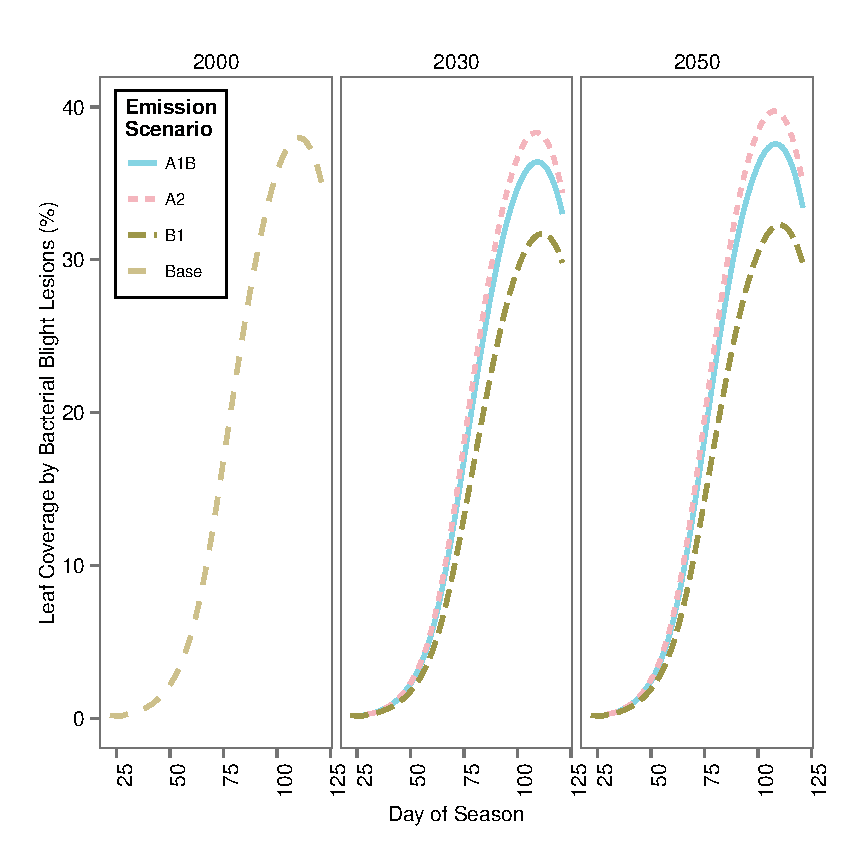
\includegraphics[width = 140mm]{figures/LB}
  \caption{Leaf blast disease severity curves as predicted by the EPIRICE model. The EPIRICE model predicts disease severity of several rice diseases using weather data inputs to predict daily disease severity and the cumulative value, AUDPC, at the end of season.}
    \label{LBCurves}
\end{figure}

% Leaf blast and bacterial blight AUDPC Table
\begin{table}[H]
\begin{tabular}{@{}lllllll@{}}
\toprule
\multicolumn{1}{c}{\begin{tabular}[c]{@{}c@{}}Emission\\ Scenario\end{tabular}} & \multicolumn{6}{c}{Time Slice} \\ \cmidrule(l){2-7} 
 & \multicolumn{3}{c}{\begin{tabular}[c]{@{}c@{}}Mean Leaf Blast\\ AUDPC\end{tabular}} & \multicolumn{3}{c}{\begin{tabular}[c]{@{}c@{}}Mean Bacterial Blight\\ AUDPC\end{tabular}} \\ \cmidrule(l){2-7} 
 & 2000 & 2030 & 2050 & 2000 & 2030 & 2050 \\ \midrule
Base & 88 &  &  & 1699 &  &  \\
A1B &  & 66 & 59 &  & 1656 & 1738 \\
A2 &  & 67 & 59 &  & 1749 & 1843 \\
B1 &  & 57 & 54 &  & 1387 & 1445 \\ \bottomrule
\end{tabular}
\caption{Area under disease progress curve values for leaf blast and bacterial blight as predicted by EPIRICE. The EPIRICE model predicts disease severity of several rice diseases using weather data inputs to predict daily disease severity and the cumulative value, AUDPC, at the end of season. A quantitative measure of disease severity over time, AUDPC allows us to compare disease severity at different times.}
\label{AUDPCTable}
\end{table}

Bacterial blight epidemics exhibited normal progress curves for the disease with a much greater severity in all time slices than that of LB. Under all time slices and scenarios the predicted epidemic started rapidly increasing around day 50 and increased up until day 100, when it began decreasing at crop maturity (Figure \ref{BBCurves}). The three different emission scenarios result in differing AUDPC responses for bacterial blight across the time slices (Table \ref{AUDPCTable}). The A2 scenario resulting in the highest predicted disease levels, the B1 scenario is notably lower than the Base or A1B or A2 scenarios.

% Bacterial blight progress curves
\begin{figure}[H]
  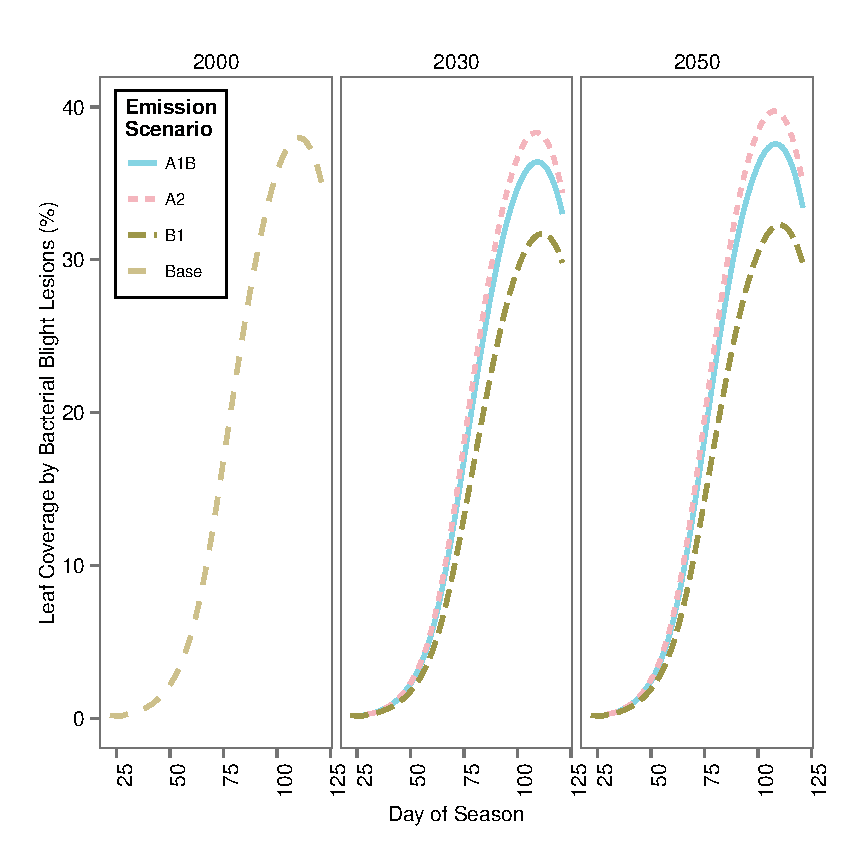
\includegraphics[width = 140mm]{figures/BB}
  \label{BBCurves}
  \caption{Bacterial leaf blight disease severity curves as predicted by the EPIRICE model. The EPIRICE model predicts disease severity of several rice diseases using weather data inputs to predict daily disease severity and the cumulative value, AUDPC, at the end of season.}
\end{figure}

\subsection{Predicted yields and yield losses (RICEPEST output)}
\subsubsection{Attainable yields}
RICEPEST predicted average attainable yields under the current conditions, in the absence of yield reducing factors, to be 0.46 tons per hectare for the current rice growing areas of Tanzania for the base climate (Figure \ref{Yield_Attainable_Violin}). Future conditions were all predicted to have higher attainable yields.

% Leaf blast yield loss violin plots
\begin{figure}[H]
  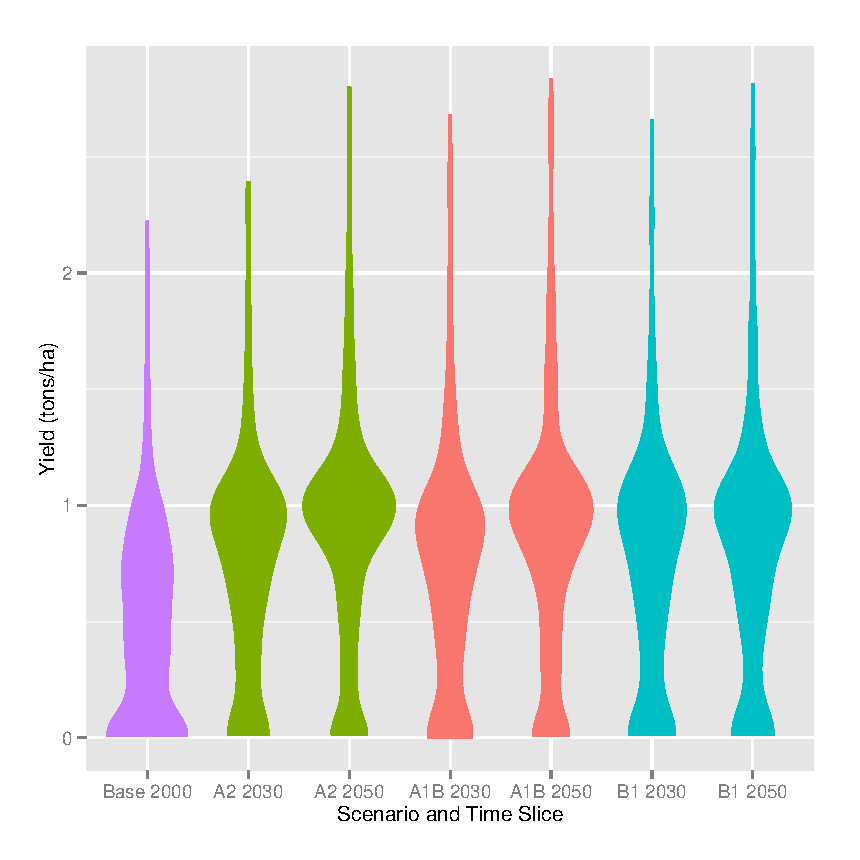
\includegraphics[width = 140mm]{figures/Yield_Attainable_Violin}
  \label{Yield_Attainable_Violin}
  \caption{RICEPEST predicted attainable yield (i.e., the yield in the absence of yield reducing factors) in tons per hectare for all time slices and emission scenarios. The RICEPEST model predicts both attainable yield and the yield in the presence of yield-reducing factors.}
\end{figure}



\subsubsection{Yield losses due to leaf blast}
Yield losses due to leaf blast were predicted to be low in Tanzania during all time slices and for all emission scenarios, the highest value for any time slice and scenario combination was 0.017 tons per hectare (Figure \ref{LB_Losses_Violin}). Differences between all time slices and scenarios were negligible, however the base had the highest yield loss values due to leaf blast, but lowest overall yield losses for the whole country. The A2 2050 scenario exhibited the highest average yield losses of any scenario and time slice combination, with the highest yield loss being 0.0169 tons per hectare for the A2 scenario during the 2030 time slice.

% Leaf blast yield loss violin plots
\begin{figure}[H]
  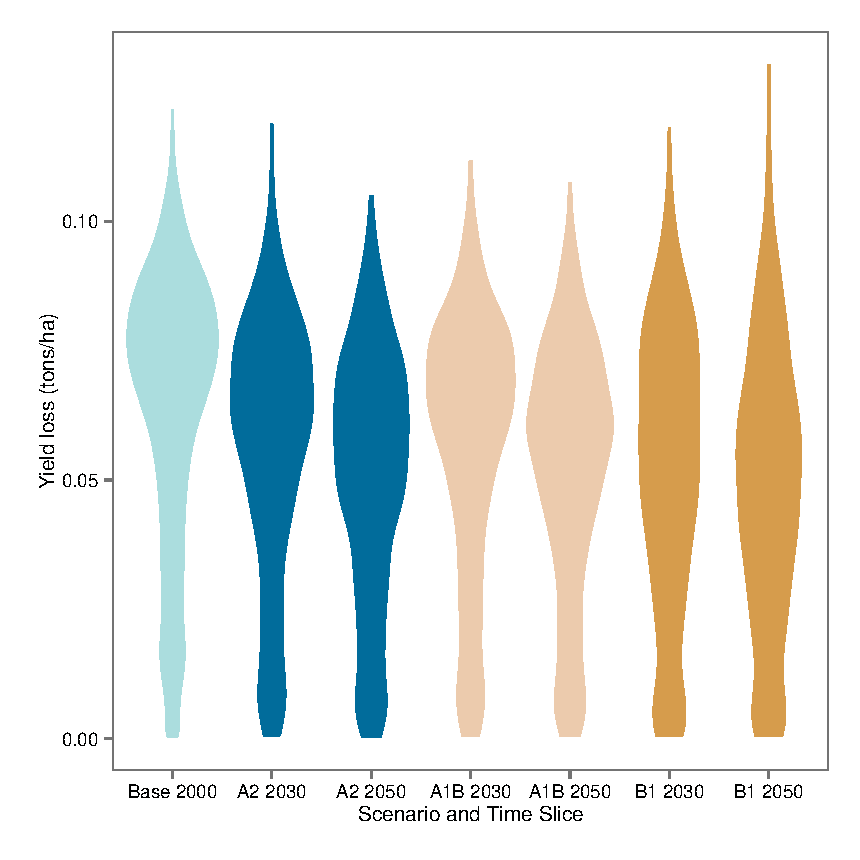
\includegraphics[width = 140mm]{figures/LB_Losses_Violin}
  \label{LB_Losses_Violin}
  \caption{RICEPEST model predicted yield loss in tons per hectare due to leaf blast for all time slices and emission scenarios. The RICEPEST model predicts both attainable yield and the yield in the presence of yield-reducing factors.}
\end{figure}

\subsubsection{Yield losses due to bacterial blight}
Bacterial blight was predicted to cause much greater losses than leaf blast (Figure \ref{BB_Losses_Violin}). The base time slice and scenario again had the lowest predicted yield losses with 0.47 tons per hectare. The A2 2050 time slice had the highest yield losses, with a maximum of 0.67 tons per hectare and an average yield loss of 0.14 tons per hectare.

% Bacterial blight yield loss violin plots
\begin{figure}[H]
  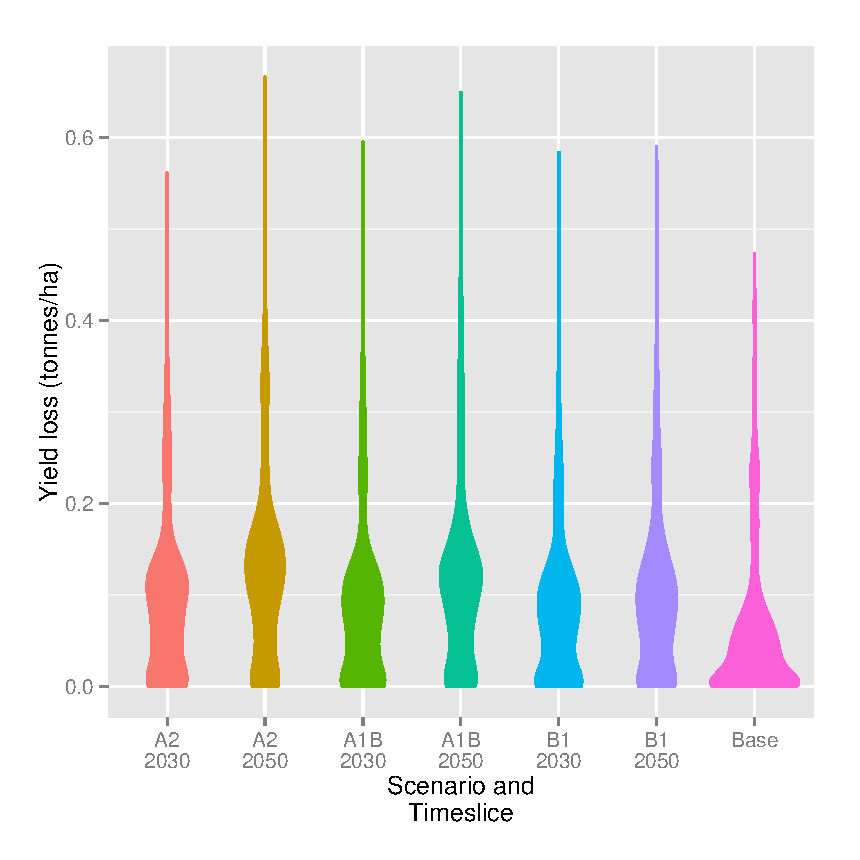
\includegraphics[width = 140mm]{figures/BB_Losses_Violin}
  \label{BB_Losses_Violin}
  \caption{RICEPEST model predicted yield loss in tons per hectare due to bacterial blight for all time slices and emission scenarios. The RICEPEST model predicts both attainable yield and the yield in the presence of yield-reducing factors.}
\end{figure}

Except for the B1 scenario time slices for leaf blast, neither disease displays a distribution of yield losses that is similar to the base time slice. The base time slice for both diseases clusters near zero, whereas the future time slices tend to have the largest concentration of values above zero, suggesting that even though the maximum values may not indicate much change, overall there is a predicted increase in the yield losses due to disease.

\citet{Burke2009} suggest that changes in climate may cause...

\citet{Thornton2009} says...

\section{Conclusions}

\section{Acknowledgments}
MICCORDEA project financed by GIZ, CCAFS and GRiSP consortium research programs


%% The Appendices part is started with the command \appendix;
%% appendix sections are then done as normal section
% \appendix



%% References
%%
%% Following citation commands can be used in the body text:
%% Usage of \cite is as follows:
%%   \cite{key}          ==>>  [#]
%%   \cite[chap. 2]{key} ==>>  [#, chap. 2]
%%   \citet{key}         ==>>  Author [#]

%% References with bibTeX database:

\bibliographystyle{elsarticle-num-names}
\bibliography{MICORDEA_References}

%% Authors are advised to submit their bibtex database files. They are
%% requested to list a bibtex style file in the manuscript if they do
%% not want to use model1-num-names.bst.

%% References without bibTeX database:

% \begin{thebibliography}{00}

%% \bibitem must have the following form:
%%   \bibitem{key}...
%%

% \bibitem{}

% \end{thebibliography}


\end{document}

%%
%% End of file `Duku et al.tex'.
